\subsection{Multi GPU Experiments}
\label{chap:methods:sec:multi}

We further evaluate LLM inference on GPUs by scaling out to multi-GPU inference.

Multi-GPU parallelism allows for expanding the evaluation in two directions: first, it enables evaluation of significantly larger models compared to single-GPU, thanks to model weight sharding across devices. This also allows a further study of performance scaling with model size. To do so, we include all the models presented in \ref{tab:models}.
Second, as discussed in Section \ref{chap:background:sec:serving}, multi-GPU inference can be implemented using several parallelization strategies, including Tensor Parallelism, Expert Parallelism, and Data Parallelism. As detailed in Section \ref{chap:methods:sec:multi}, these techniques increase the system’s parallel throughput and memory bandwidth approximately linearly with the number of accelerators. Combining these methods introduces a trade-off between the lower communication overhead of Data Parallelism and the greater available memory provided by Tensor Parallelism.

\begin{figure}[h!]
    \centering
    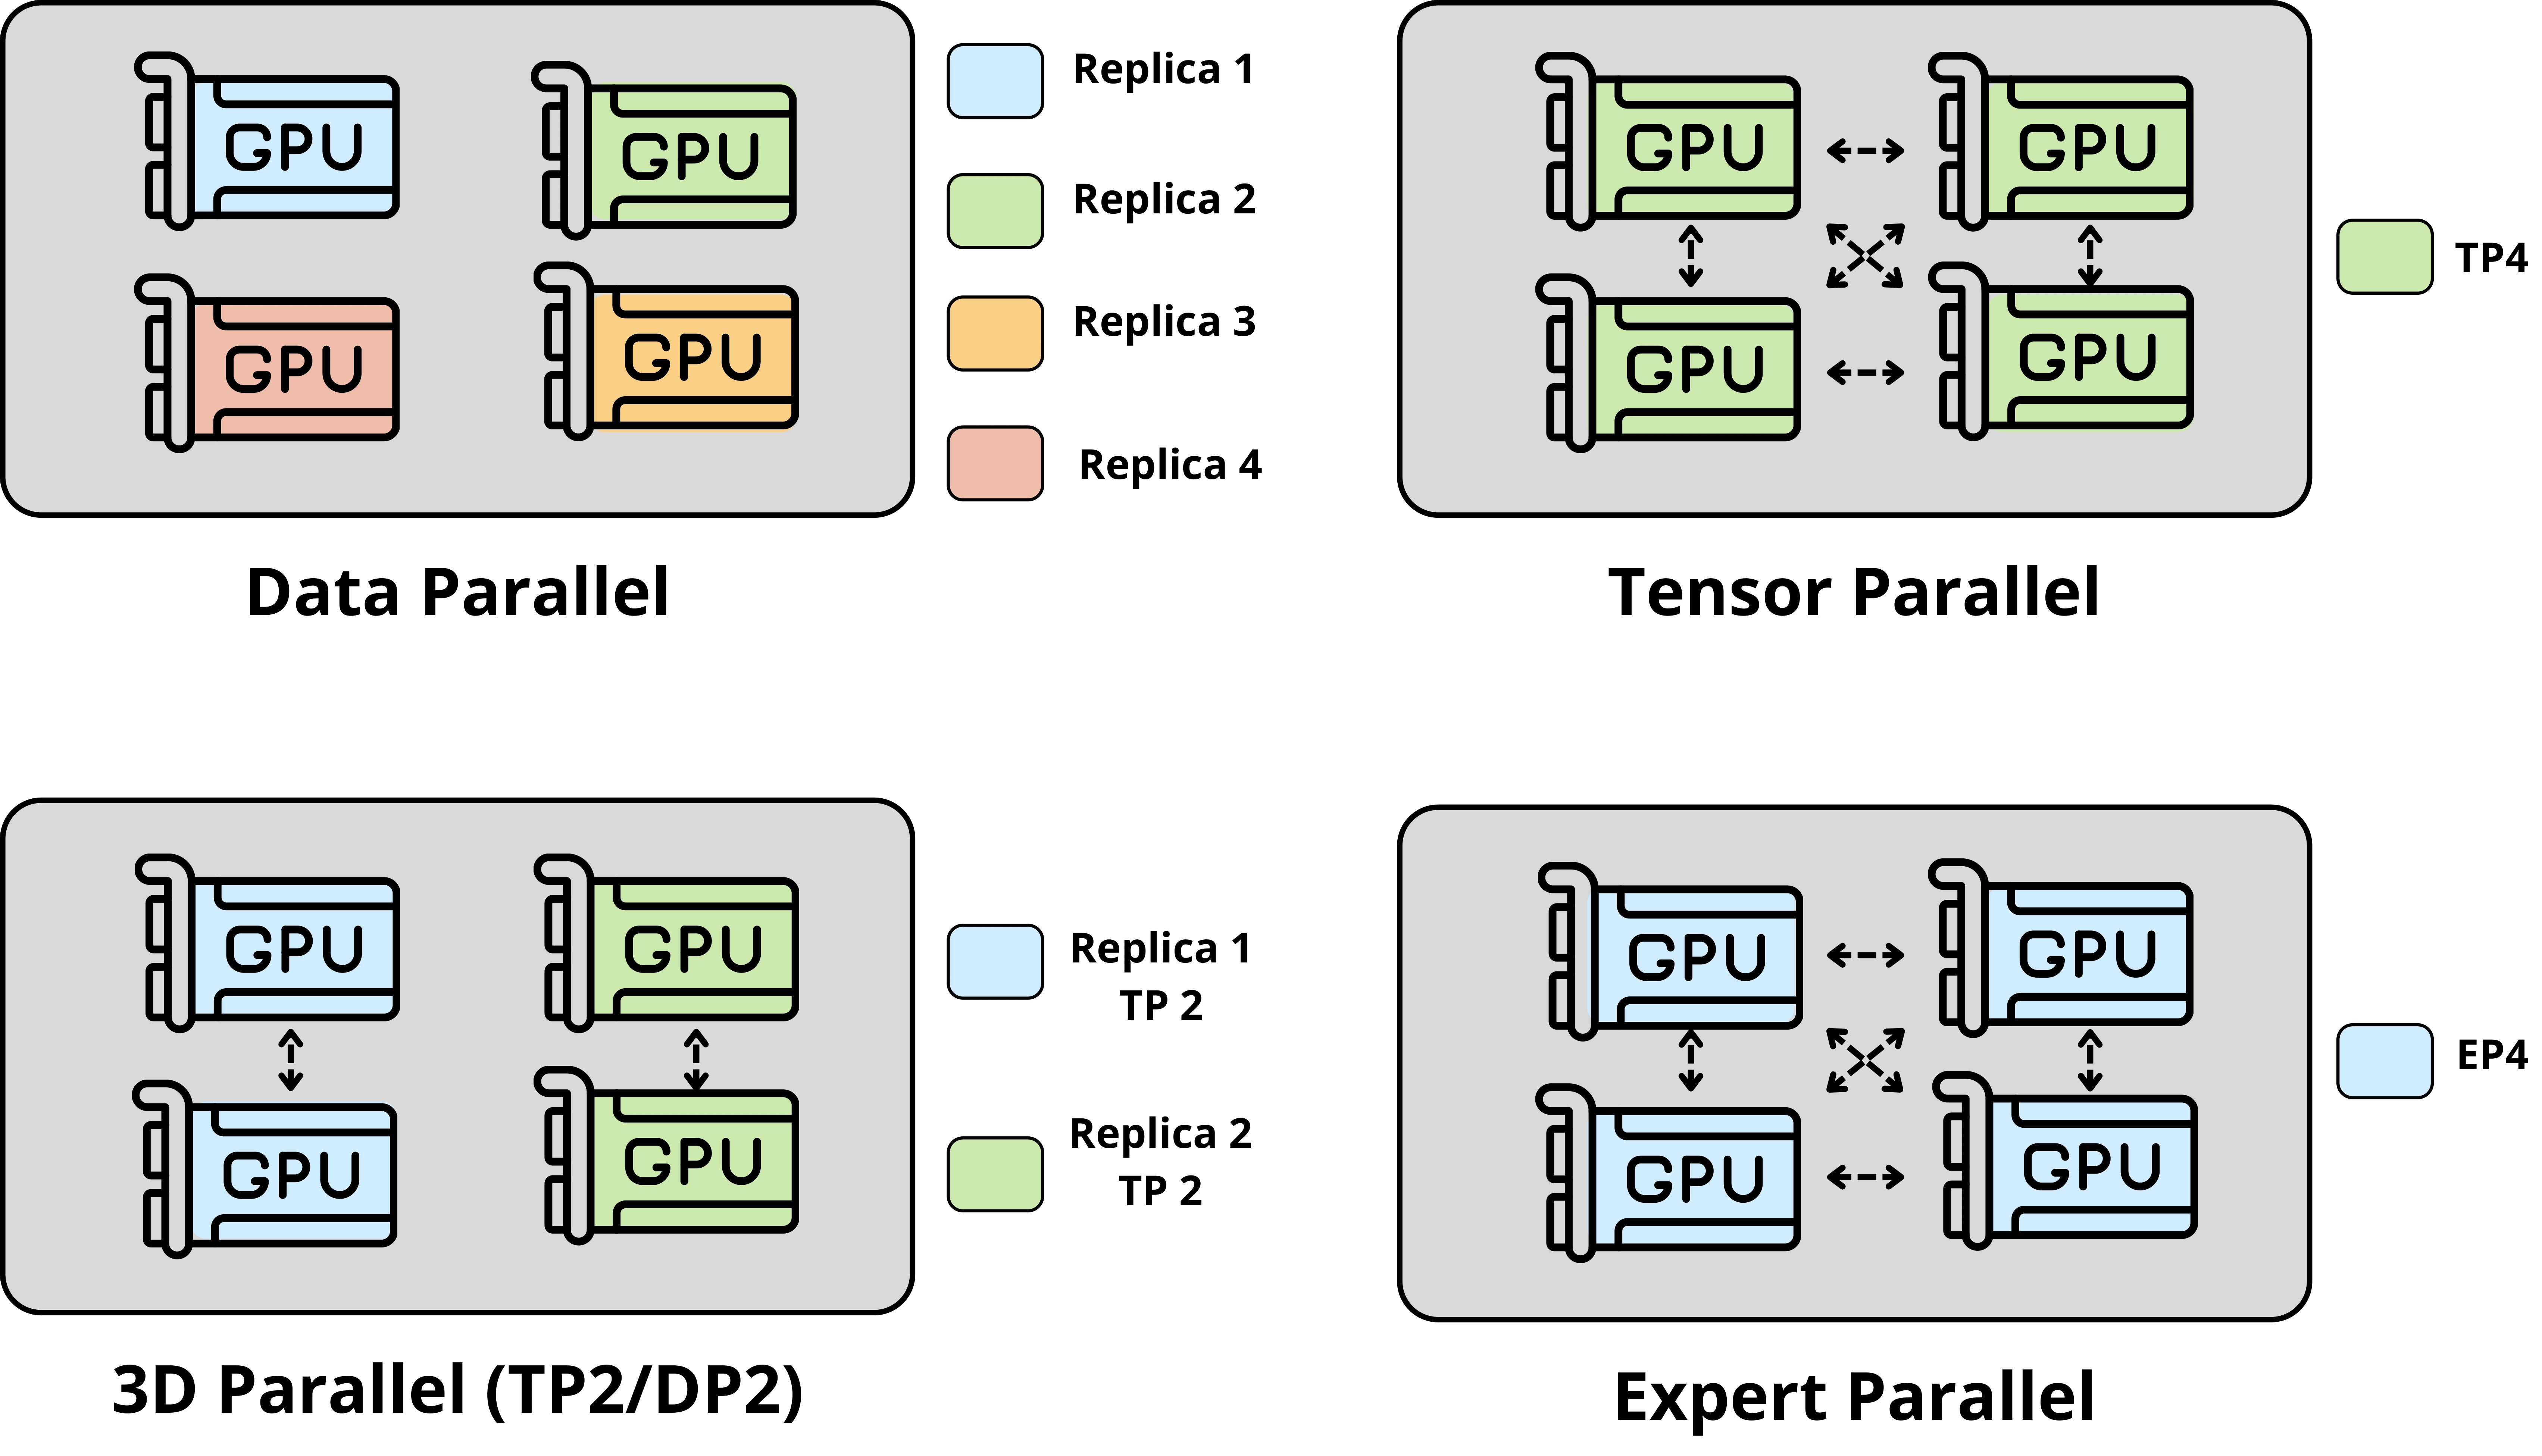
\includegraphics[width=0.85\textwidth]{figs/partition.png}
    \vspace{5mm}
    \caption{Partitioning a node with 3D parallelism.}
    \tagpdfsetup{alttext={Partitioning a node with 3D parallelism.}}
    \label{fig:partition}
\end{figure}

Achieving optimal node-level performance thus requires balancing the number of Data Parallel (DP) replicas and the Tensor Parallel (TP) width per instance, depending on the model size and hardware characteristics. In this study, we explore various TP/DP configurations to empirically determine near-optimal settings. \ref{fig:partition} shows multiple options for partitioning the resources of a 4-GPU node.

\begin{figure}[h!]
    \centering
    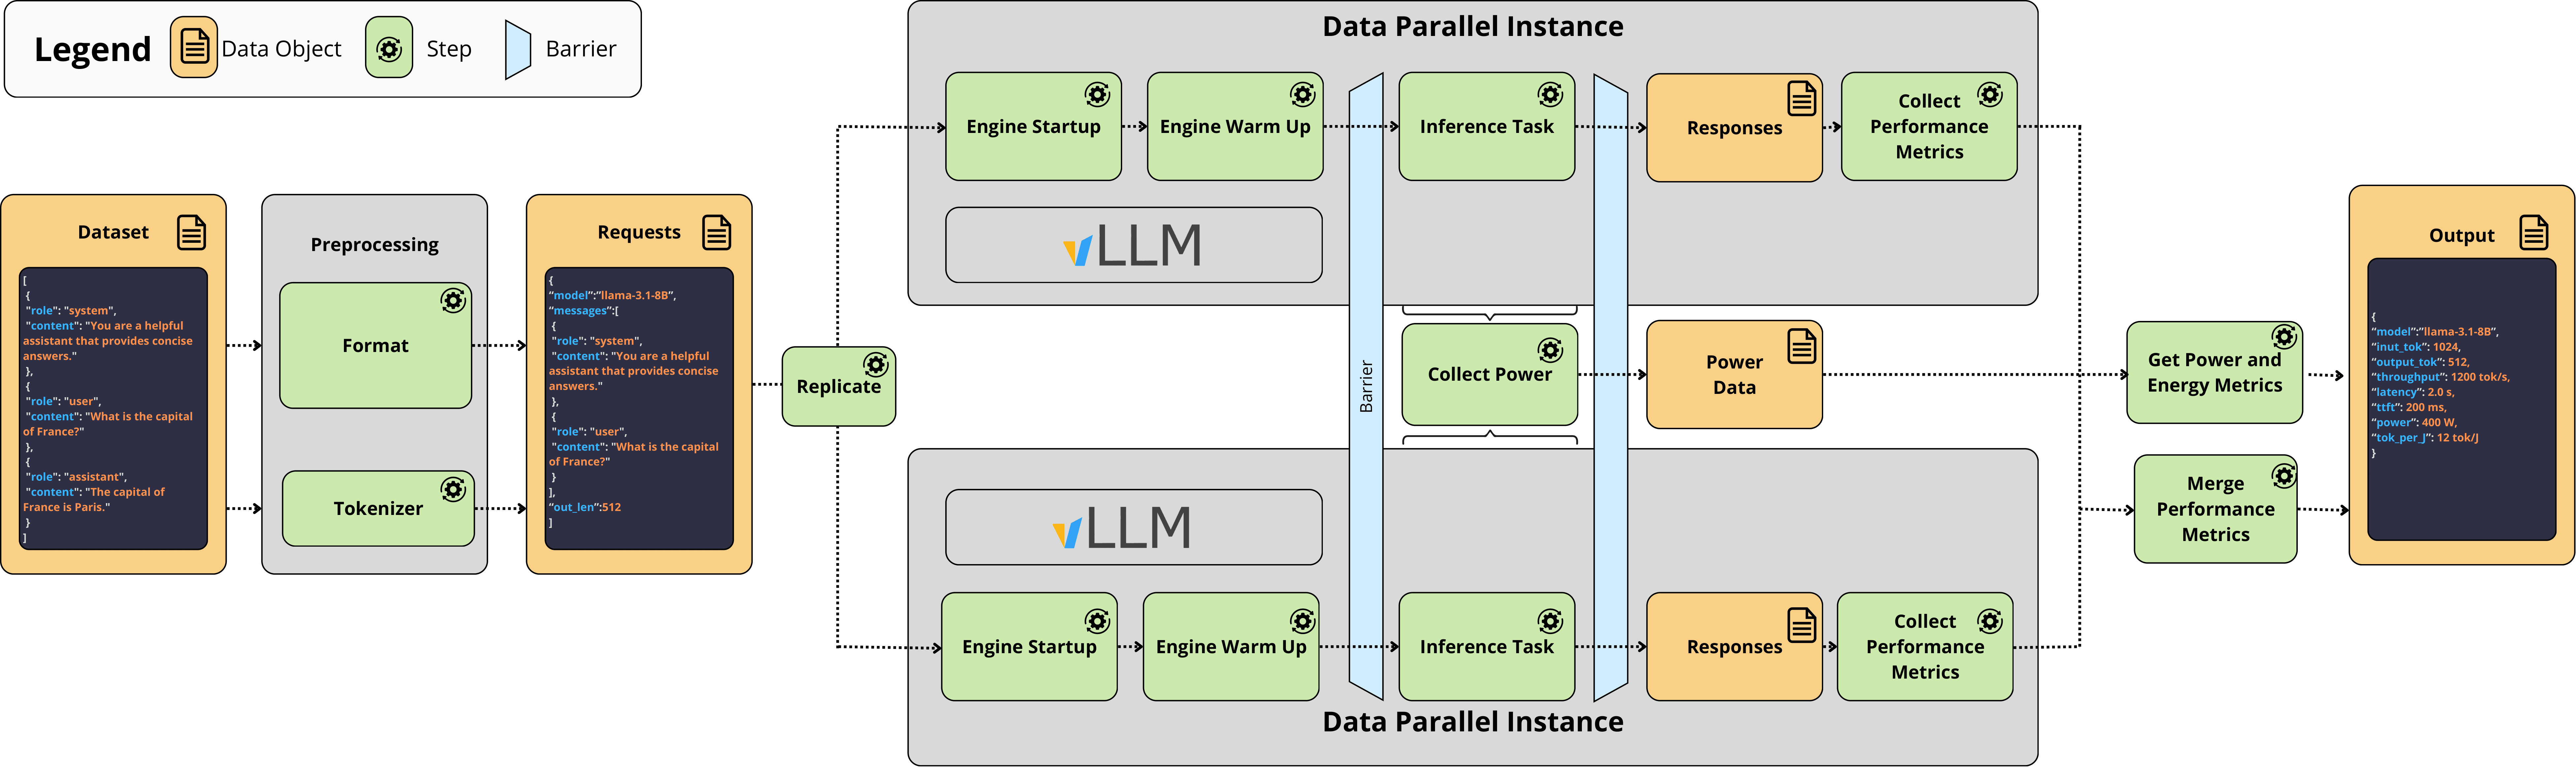
\includegraphics[width=\textwidth]{figs/profile multi.png}
    \vspace{5mm}
    \caption{LLM Inference Benchmark Stages. Multi-GPU setup.}
    \tagpdfsetup{alttext={LLM Inference Benchmark Stages. Multi-GPU setup.}}
    \label{fig:bench}
\end{figure}

An experiment with Data Paralle Size $D$ and Tensor Parallel Size $T$ begins by creating $D$ worker processes and one profiler process. Similar to the single-GPU setup, the profiler process probes the vendor-specific system monitoring interface at consistent intervals to retrieve power consumption data.
Each worker process, instead, initiates a vLLM instance with Tensor Parallel Size $T$. Setting $T\times D = N$, where $N$ is the number of GPUs of the node, allows for an even partition into $D$ homogenous portions, as shown by \ref{fig:partition}.

Once all the $D$ instances are ready, each one starts processing a full instance of the dataset, scaling the single-GPU experiment weakly. When all instances have finished generating replies, their outputs are combined to extract performance metrics, and the profiler process is terminated.

We repeat this experiment with Tensor Parallel Size $T \in \{1, 2, 4\}$ on three multi-GPU nodes: one Sophia bigmem node, featuring 8 DGX A100 80GB GPUs, and two JLSE testbed nodes, featuring 4 NVIDIA H100 SXM5 and 8 AMD Instinct MI300X, respectively. The Data Parallel Size $D$ is set to fully utilize the node. 
The global batch size is set to $128 \times N$, meaning that each of the $D$ instances has a batch size of $128\times T$.
We evaluate both bfloat16 precision and FP8 quantization, using W8A8 on Nvidia H100 and AMD MI300x, and W8A16 on Nvidia A100.

These weak scaling settings allow us to have cleaner performance scaling in two ways. First, it maintains consistency in context lengths across data-parallel instances, since all replicas process identical sequences. Second, it maintains a constant batch size per GPU, ensuring that the number of generated tokens per forward pass remains unchanged across different TP/DP configurations.

\subsection{Comparing Tensor and Expert Parallelism}

We further investigate parallelization strategies for Mixture-of-Experts (MoE) models by comparing Tensor Parallelism (TP) and Expert Parallelism (EP).

Our evaluation includes four large MoE models — Llama4 Scout, Mixtral 8×22B, Qwen 235B A22B, and DeepSeek R1 — all tested in FP8 precision on NVIDIA H100 and AMD MI300x nodes.

Experiments are conducted across varying batch sizes, using a single instance (Data Parallel size = 1) with four GPUs per instance. We first test with a Tensor Parallel size of 4, followed by an Expert Parallel size of 4. The profiling methods used are consistent with those employed in the previous experiment. For DeepSeekR1, we also experimented with 8 GPUs.
